\documentclass[tikz,border=10pt]{standalone}
%\usepackage{fontspec}
\usepackage{amsmath}
\usetikzlibrary{arrows.meta, positioning, shadows.blur}

% Define colors
\definecolor{datacolor}{RGB}{70,130,180}      % Steel blue
\definecolor{aicolor}{RGB}{220,100,60}        % Coral/orange
\definecolor{expcolor}{RGB}{50,160,50}        % Green
\definecolor{feedbackcolor}{RGB}{140,100,180} % Purple

\tikzset{
  block/.style={
    rectangle,
    rounded corners,
    minimum width=4.5cm,
    minimum height=1.4cm,
    text centered,
    draw=black,
    thick,
    blur shadow={shadow blur steps=3},
    font=\small
  },
  arrow/.style={
    ->,
    >=Stealth,
    thick
  },
  feedback/.style={
    ->,
    >=Stealth,
    thick,
    feedbackcolor,
    dashed
  }
}

\begin{document}

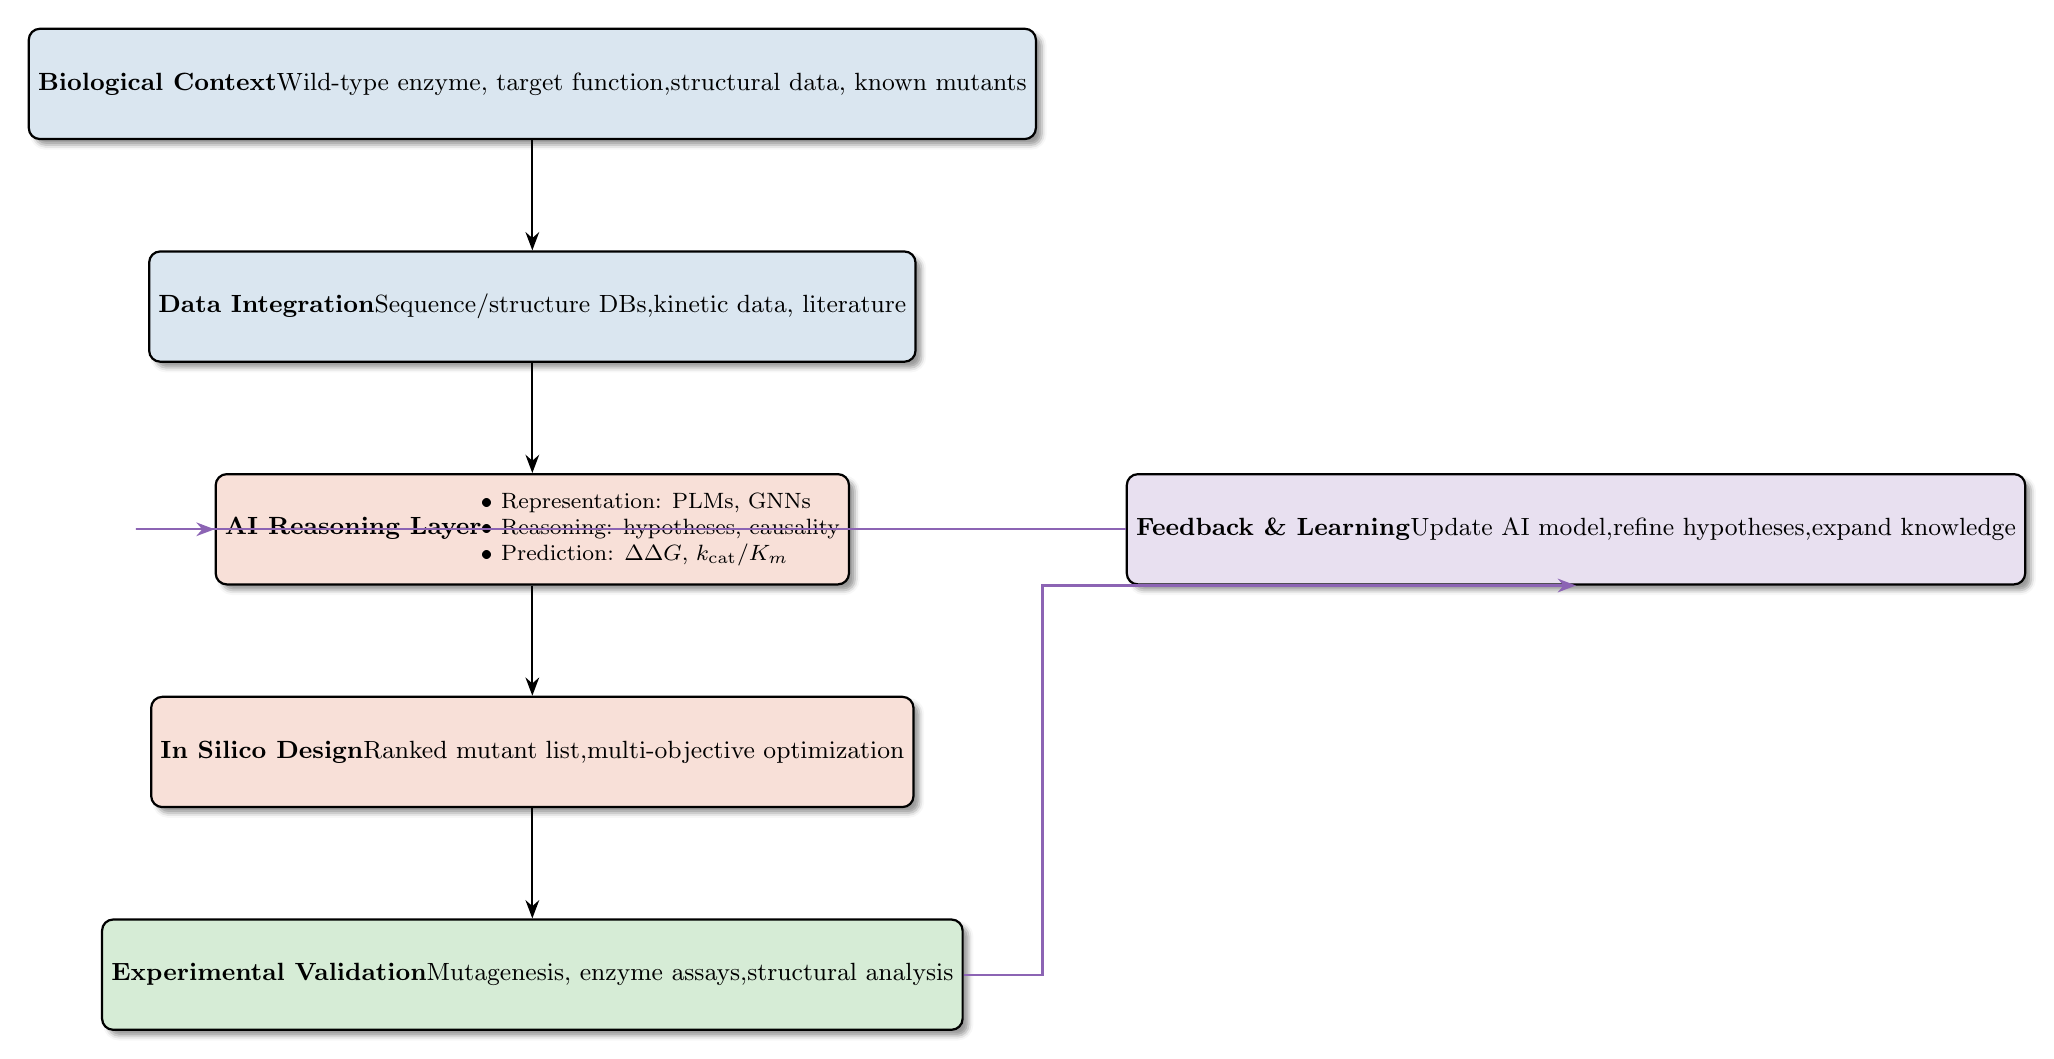
\begin{tikzpicture}[node distance=1.4cm and 2cm]

% Nodes
\node[block, fill=datacolor!20] (context) {
  \textbf{Biological Context} \\
  Wild-type enzyme, target function, \\
  structural data, known mutants
};

\node[block, fill=datacolor!20, below=of context] (data) {
  \textbf{Data Integration} \\
  Sequence/structure DBs, \\
  kinetic data, literature
};

\node[block, fill=aicolor!20, below=of data] (ai) {
  \textbf{AI Reasoning Layer} \\
  \footnotesize
  \begin{tabular}{@{}l@{}}
    • Representation: PLMs, GNNs \\
    • Reasoning: hypotheses, causality \\
    • Prediction: $\Delta\Delta G$, $k_{\text{cat}}/K_m$
  \end{tabular}
};

\node[block, fill=aicolor!20, below=of ai] (design) {
  \textbf{In Silico Design} \\
  Ranked mutant list, \\
  multi-objective optimization
};

\node[block, fill=expcolor!20, below=of design] (exp) {
  \textbf{Experimental Validation} \\
  Mutagenesis, enzyme assays, \\
  structural analysis
};

\node[block, fill=feedbackcolor!20, right=3.5cm of ai] (feedback) {
  \textbf{Feedback \& Learning} \\
  Update AI model, \\
  refine hypotheses, \\
  expand knowledge
};

% Vertical arrows
\draw[arrow] (context) -- (data);
\draw[arrow] (data) -- (ai);
\draw[arrow] (ai) -- (design);
\draw[arrow] (design) -- (exp);

% Feedback loop
\draw[arrow, feedbackcolor] (exp.east) -| ([xshift=1cm]exp.east) 
    |- node[pos=0.25, right, black] {} (feedback.south);
\draw[arrow, feedbackcolor] (feedback.west) -| ([xshift=-1cm]ai.west) -- (ai.west);

% Optional: Add icons or labels (commented for simplicity)
% \node[above=0.1cm of context, font=\large] {\faFlask}; % requires fontawesome

\end{tikzpicture}

\end{document}
